%!TEX root=seke.tex
% mainfile: seke.tex

\documentclass[10pt,twocolumn]{article}

\usepackage{moreverb}
\usepackage{graphicx}
\usepackage[utf8]{inputenc}
\usepackage[T1]{fontenc} 
\usepackage{multirow}
\usepackage{algorithm}
\usepackage{algpseudocode}
\usepackage{pifont} 
\usepackage{import}
\usepackage{amsmath}
\usepackage[table]{xcolor}% http://ctan.org/pkg/xcolor
\usepackage{latex8}
\usepackage{times}
\usepackage{inconsolata}
\usepackage{pifont}
\usepackage{placeins}
\usepackage{adjustbox}
\usepackage{lipsum}
\usepackage{textcomp}
\usepackage{listings}
\usepackage{caption}
\usepackage{amsmath}
\usepackage{calc} 
\usepackage{array,url,kantlipsum}
\usepackage{algorithm}
\usepackage{algpseudocode}
\usepackage{lscape}
\usepackage{array}
\usepackage{longtable}
\usepackage{booktabs}
\usepackage{txfonts}

\usepackage{graphicx}
\usepackage{algorithm}
%\usepackage{algorithmic}

\usepackage{tikz}
\usetikzlibrary{shapes,arrows,shadows}
\usepackage{amsmath,bm,times}
\usepackage{verbatim}

\usepackage{subcaption}
\usepackage{bibspacing}
\usepackage{fancyhdr}

\renewcommand*\thelstnumber{\arabic{lstnumber}:}

\DeclareCaptionFormat{mylst}{\hrule#1#2#3}
\captionsetup[lstlisting]{format=mylst,labelfont=bf,singlelinecheck=off,labelsep=space,font={normalsize,tt}}

\usepackage[dvips,colorlinks,bookmarksopen,bookmarksnumbered,citecolor=red,urlcolor=red]{hyperref}


\renewcommand{\headrulewidth}{0pt}
\fancypagestyle{doi}{\lfoot{DOI reference number: 10.18293/SEKE2015-205}}

\usepackage[small,compact]{titlesec}
% \usepackage{titlesec}

\pagenumbering{gobble}

\newcommand{\goallegheny}{$^{\mbox{\footnotesize \ding{72}}}$}
\newcommand{\gosheffield}{$^{\mbox{\footnotesize \ding{73}}}$}
\newcommand{\gospace}{$\;$}



% \makeatletter
% \renewenvironment{thebibliography}[1]{%
%   \vspace*{-.1in}
%   \@xp\section\@xp*\@xp{\refname}%
%   % \normalfont\footnotesize\labelsep .5em\relax
%   \renewcommand\theenumiv{\arabic{enumiv}}\let\p@enumiv\@empty
%   \vspace*{-.1in}% NEW
%   \list{\@biblabel{\theenumiv}}{\settowidth\labelwidth{\@biblabel{#1}}%
%     \leftmargin\labelwidth \advance\leftmargin\labelsep
%     \usecounter{enumiv}}%
%   % \sloppy \clubpenalty\@M \widowpenalty\clubpenalty
%   % \sfcode`\.=\@m
% }{%
%   \def\@noitemerr{\@latex@warning{Empty `thebibliography' environment}}%
%   \endlist
% }
% \makeatother

\begin{document}

% \title{Empirically Evaluating the Efficiency of Search-based \\ Test Data
% Generation for Relational Database Schemas\vspace*{-.1in}}

\title{\vspace*{-.6in}Implementing a testbed tool for \\ load, performance and stress search based tests\vspace*{-.1in}}

\author{Nauber Gois, Pedro Porfírio, André Coelho
      }

\affiliation{Universidade de Fortaleza, UNIFOR, Av. Washington Soares, 1321 , Fortaleza - CE,  Brazil
}

\email{naubergois@gmail.com}

\maketitle

\thispagestyle{doi}

\begin{abstract}

% When evaluating an algorithm, it is often useful to speak of it's efficiency in terms of it's worst-case complexity.
% This is the case for search-based test data generation tools.
% on the search-based data generation tool \textit{SchemaAnalyst}.

% This paper introduces a framework for conducting automated empirical studies of algorithms by doubling
% the size of the input and observing the change in runtime.

% After describing a way to systematically doubling the size of structured data, we report on a study demonstrating the
% presented method's effectiveness.

Metaheuristic search techniques have been extensively used to provide solutions for a more cost-effective testing process. The use of metaheuristic search techniques for the automatic generation
of test  has been a burgeoning interest for many researchers in recent years. Search Based Software Testing refers to the use of meta-heuristics for the optimization of a task in the context of
software testing. Experimentation is important to realistically and accurately
test and evaluate search based tests. Experiments involving stress search based tests are inherently complex and typically time-consuming to set up and
execute. Such experiments are also extremely difficult to
repeat, People who might want to duplicate published results, for example, must devote substantial resources to setting up and the environmental conditions are likely to be substantially different. A Testbed makes possible follow a formalized it's a methodology to reproduce tests for further analysis and comparison. Since a real testbed is often extremely costly, an open source testbed simulator can represent a valid alternative to real device development and testbed deployment for academic and industrial research goals. In this paper, we propose a testbed tool named IAdapter TestBed to evaluate various diversity combining metaheuristics in search-based software testing. Two experiments were conducted to validate the proposed tool. In the first experiment the metaheuristics converged to scenarios with no antipatterns. In the second experiment,  the metaheuristics excluding the scenarios with Unbalanced Processing antipattern.

\end{abstract}

%!TEX root=../seke.tex
% mainfile: ../seke.tex

\vspace*{-.15in}
\section{Introduction}
\vspace*{-.05in}

Performance problems such as high response times in software applications have a significant effect on the customer’s satisfaction. The explosive growth of the Internet has contributed to the increased need for applications that perform at an appropriate speed. Performance problems are often detected late in the application life cycle, and the later they are discovered, the greater the cost to fix them. The use of stress testing is an increasingly common practice owing to the increasing number of users. In this scenario, the inadequate treatment of a workload generated by concurrent or simultaneous access due to several users can result in highly critical failures and negatively affect the customers perception of the company \cite{Draheim2006b} \cite{Jiang2010} \cite{Molyneaux2009} \cite{Wert2014}. 

The use of stress testing is an increasingly common practice owing to the increasing number of users. In this scenario, the inadequate treatment of a workload generated by concurrent or simultaneous access due to several users can result in highly critical failures and negatively affect the customers perception of the company \cite{Draheim2006b} \cite{Jiang2010}. 

Stress software testing is a expensive and difficult activity. The exponential
growth in the complexity of software makes the cost of testing has only continued to rise. Test case generation can be seen as a search problem. The test adequacy criterion is transformed into a fitness function and a set of solutions in the search
space are evaluated with respect to the fitness function using a metaheuristic search technique. Search-based software testing is the application of metaheuristic search techniques to generate software
tests cases or perform test execution \cite{Afzal2009a} \cite{Gay}.


Stress Search-based testing is seen as a promising approach to verifying timing constraints \cite{Afzal2009a}. A common objective of a stress search-based test is to find  scenarios that produce execution times that violate the specified timing constraints \cite{Sullivan}. 

Experiments involving stress search based tests are inherently complex and typically time-consuming to set up and
execute. Such experiments are also extremely difficult to
repeat. People who might want to duplicate published results, for example, must devote substantial resources to setting up and the environmental conditions are likely to be substantially different. Comparing a new metaheuristic to existing ones, it is advantageous to test on the problem instances already tested by previous papers. Then, results will be comparable on a by-instance basis, allowing relative gap calculations between the two heuristics. A Testbed makes possible follow a formalized methodology and reproduce tests for further analysis and comparison. It seems natural that one of the most important parts of a comparison among heuristics is a testbed\cite{GendreauMichelandPotvin2010}.

This paper addresses the problem of comparing the use of several metaheuristics in search based tests. In this paper, we propose a flexible testbed tool to evaluate various diversity combining metaheuristics in search based software testing. A tool named IAdapter (github.com/naubergois/newiadapter), a JMeter plugin for performing search-based load tests, was extended \cite{Gois2016}. The IAdapter Testbed is an open-source tool that provides  tools for search based test research. This tool emulates test scenarios in a controled environment using mock objects and implementing performance antipatterns. Differently from patterns, antipatterns look at the negative features of a software system and describe commonly occurring solutions to problems that generate negative consequences.

Two experiments were conducted to validate the proposed tool. The experiments uses genetic, algorithms, tabu search, simulated annealing and an hybrid approach proposed by Gois et al. \cite{Gois2016}.

The remainder of the paper is organized as follows. Section 2 presents a brief introduction about load, performance, and stress tests. Section 3 presents concepts about the workload model. Section 4 presents details features about common performance antipatterns. Section 5 presents concepts about search based tests. Section 6 presents concepts about metaheuristic algorithms. Section 7 presents concepts about IAdapter Testbed. Section 8 shows the results of two experiments performed using the IAdapter plugin.  Conclusions and further work are presented in Section 10.

%!TEX root=seke.tex
% mainfile: ../seke.tex

\section{Background}

Stress testing projects should start with the development of a model for user workload that an application receives. This should take into consideration various performance aspects of the application and the infrastructure that a given workload will impact. A workload is a key component of such a model. The term workload represents the size of the demand that will be imposed on the application under test in an execution. The metric  used for measure a workload is dependent on the application domain, such as the length of the video in a transcoding application for multimedia files or the size of the input files in a file compression application \cite{Molyneaux2009}. 

Search-Based Testing is the process of automatically
generating test according to a test adequacy criterion,encoded as a fitness function, using search-based optimization algorithms, which are guided by a fitness function. The role of the fitness function is to capture a test objective that, when achieved, makes a contribution to the desired test adequacy criterion . Search–Based Testing uses metaheuristic algorithms to
automate the generation of test inputs. Metaheuristics are strategies that guide the search process to efficiently explore the search space in order to find optimal solutions  \cite{Afzal2009a}.

A common goal of stress search-based testing is to find workloads that produce execution times that exceed the timing constraints specified. If a temporal error is found, the test was successful. The application of evolutionary algorithms to  stress tests involves finding the best- and worst-case execution times (B/WCET) to determine whether timing constraints are fulfilled \cite{Afzal2009a}. 

IAdapter is a JMeter plugin designed to perform search-based stress tests. The plugin uses genetic algorithms, tabu search and simulated annealing in a collaborative mode (hybrid metaheuristic) \cite{Gois2016}. JMeter is a desktop application designed to test and measure the performance and functional behavior of applications. The JMeter tool can test an emulated class using Mock objects. A mock object is a dummy implementation for an interface or a class. A Mock Object is a substitute implementation for emulating other domain code. Basic mock object allows testing a unit faking the communication with collaborating objects. It should be simpler than the real code, not duplicate its implementation \cite{Brown2003}. 


% \vspace*{-.05in}
\section{Common performance application problems and performance antipatterns}
\vspace*{-.05in}

Performance is critical to the success of today’s software systems. Many software products fail to meet their performance objectives when they are initially constructed. There are several antipatterns that detailed features about  common performance problems. Antipatterns are conceptually similar to patterns in that they document recurring solutions to common design problems. They are known as
antipatterns because their use produces negative consequences.  Performance antipatterns document common performance mistakes made in software architectures or designs \cite{brown1998antipatterns}. Table \ref{antipatterns} present some of the most common performance antipatterns.

% Please add the following required packages to your document preamble:
% \usepackage{multirow}
% \usepackage[table,xcdraw]{xcolor}
% If you use beamer only pass "xcolor=table" option, i.e. \documentclass[xcolor=table]{beamer}
\begin{table}[h]
\centering
\caption{Performance antipatterns}
\label{antipatterns}
\begin{tabular}{|c|}
\hline
\rowcolor[HTML]{C0C0C0} \textbf{Antipattern}  \\ \hline
Blob or The God Class   \\ \cline{1-1}
Unbalanced-Processing \\ \cline{1-1}
Circuitous Treasure Hunt   \\ \cline{1-1}
Empty Semi Trucks   \\ \cline{1-1}
Tower of Babel   \\ \cline{1-1}
One-Lane Bridge   \\ \cline{1-1}
Excessive Dynamic Allocation   \\ \cline{1-1}
Traffic Jam   \\ \cline{1-1}
The Ramp    \\ \cline{1-1}
More is Less  \multirow{-10}{*}{} \\ \hline
\end{tabular}
\end{table}

Four antipatterns were chosen to this research  by the simplicity of implementation: Unbalanced-Processing, Circuitous Treasure Hunt, Tower of Babel and The Ramp.


A characteristic of Unbalanced Processing is the tendency to overload a particular resource. The overloaded resource will be executing a certain type of job very often, thus in practice, damaging other classes
of jobs that will experience very long waiting times.  Figure \ref{fig:unbalanced}  shows a sample of the Unbalanced Processing. In The Fig. \ref{fig:unbalanced}, four tasks are performed. The task D it is waiting for the task C conclusion that are submmited to a heavy processing situation. 


\begin{figure}[h]
\centering
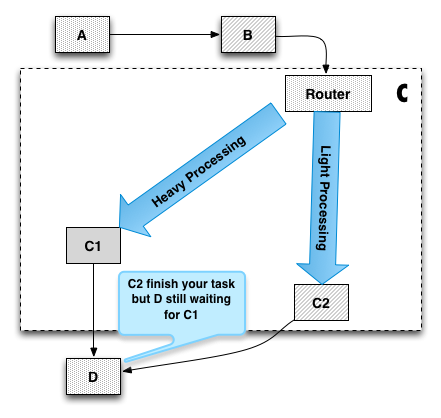
\includegraphics[width=0.4\textwidth]{./images/unbalanced.png}
\caption{Unbalanced Processing sample \cite{Wert2013a}. }
\label{fig:unbalanced}
\end{figure}

Circuitous Treasure Hunt antipattern occurs when software retrieves data from a first componet, uses those results in a second component, retrieves data from the second component, and so on, until the last results are obtained. Circuitous Treasure Hunt 
are typical performance antipatterns that causes unnecessarily high amount of frequent database requests \cite{Wert2014}. 

Tower of Babel antipattern most often occurs when information is translated into an exchange format, such as XML, where the sending process is then parsed and translated into an internal format by the receiving process. When the translation and parsing is excessive, the system spends most
of its time doing this \cite{Wert2014}.

\begin{figure}[h]
\begin{minipage}{.5\textwidth}
\centering
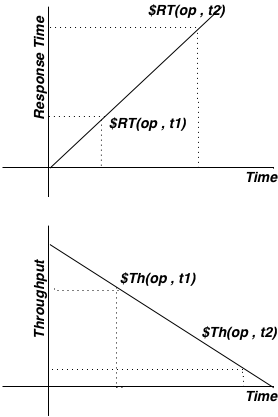
\includegraphics[width=0.5\textwidth]{./images/ramp.png}
\caption{The Ramp sample \cite{Vetoio2011}.}
\label{fig:ramp}
\end{minipage}
\end{figure}

Ramp is an antipattern where the processing time increases as the system is used. Fig. \ref{fig:ramp} shows a system  with the Ramp problem:  (i) the monitored response time of the operation opx at time t1, i.e. \$RT(opx, t1), is much lower than at time t2, i.e. \$RT(opx, t2), with t1 < t2; (ii) the monitored throughput of the operation opx at time t1, i.e. \$Th(opx, t1), is much larger than at time t2, i.e. \$Th(opx, t2), with t1 < t2 \cite{Wert2014}. 
%!TEX root=seke.tex
% mainfile: ../seke.tex

\vspace*{-.075in}
\section{The IAdapter Testbed system}\label{sec:technique}
\vspace*{-.075in}


In this section, We devise a new testbed that has the ability to reproduce different types of web workloads.  The proposed solution extends a tool named IAdapter to create a testbed tool to validade load, performance and stress search based test approaches \cite{Gois2016}. This new testbed must accomplish three main goals. First, it must reproduce a workload by using an antipattern implementation. Second, it must be able to provide metrics with the aim of being used for research evaluation studies. Finally, it should be extensible, allowing the creation of new metaheuristic approaches.

The testbed tool proposed consists of four main modules.  Figure \ref{fig:testbedarch} presents the main architecture of the Testbed solution proposed. The emulator module provides workloads to the Test module. The Test module uses a class loader to find all classes that extends AbstractAlgorithm in the classpath and run all workloads with each metaheuristic found. The Test Scenario library provides the scenario representation used by the metaheuristics and store the testbed results in a database. The Operation services are responsible for finding neighbors of some workload provided as a parameter and perform crossover operations.

\begin{figure}[h]
\centering
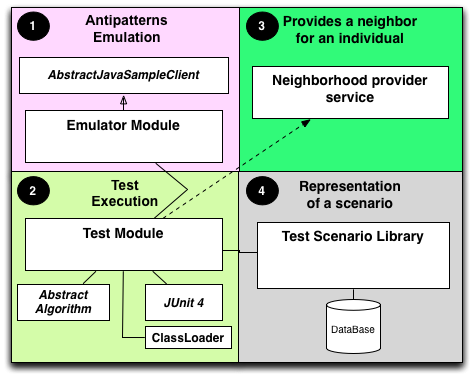
\includegraphics[width=0.5\textwidth]{./images/testbedarch.png}
\caption{Testbed main architecture.}
\label{fig:testbedarch}
\end{figure} 

\begin{figure}[h]
\centering
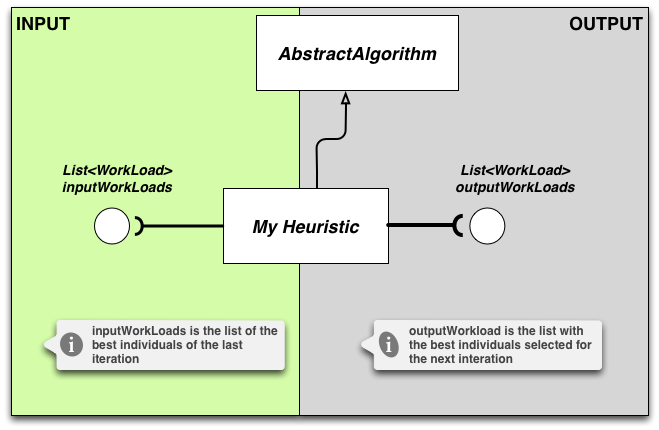
\includegraphics[width=0.5\textwidth]{./images/myheuristic.png}
\caption{Test Module class diagram.}
\label{fig:heuristicclassdiagram}
\end{figure} 



\subsection{Test Module}

The Test Module (Figure \ref{fig:testbedarch}  -\ding{202}) is responsible for for the loading of all classes that extend AbstractAlgorithm in the classpath and perform the tests under the application. Figure \ref{fig:heuristicclassdiagram} shows the  class diagram for custom and provided heuristics. All heuristic classes extends the class AbstractAlgorithm. The heuristics receives  as input a  list of workloads (Figure \ref{fig:heuristicclassdiagram}  -\ding{203}) and must return a list of output workloads (the individuals selected for the next generation)  (Figure \ref{fig:heuristicclassdiagram}  -\ding{204}). Each workload represent an individual in the search space. Figure. \ref{fig:step2} presents the Test Module life cycle. Given an initial population (Figure \ref{fig:step2}  -\ding{202}),  a metaheurist select a new set of workloads based on an objective function (Figure \ref{fig:step2}  -\ding{203}). The choosen metaheurist generate a new set of individuals based on crossover or neighborhood operators (Figure \ref{fig:step2}  -\ding{204}).  JMeterEngine run each workload (Figure \ref{fig:step2}  -\ding{206}) and the choosen metaheuristic obtain a fitness value for each workload based on some objective function  (Figure \ref{fig:step2}  -\ding{207}). Each Metaheuristic could define your own objective function. After all these steps the cycle begins until the maximum number of generations it is reached (Figure \ref{fig:step2}  -\ding{208}). 

\begin{figure}[h]
\begin{minipage}{.5\textwidth}
\centering
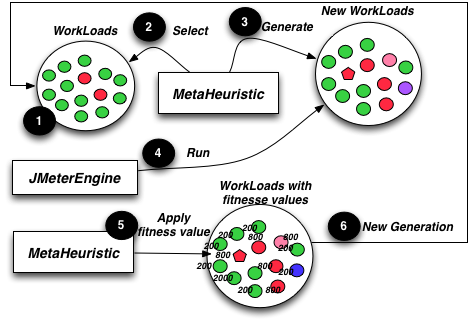
\includegraphics[width=1\textwidth]{./images/step2.png}
\caption{Test module life cycle.}
\label{fig:step2}
\end{minipage}
\end{figure} 



\subsection{Emulator Module}

The Emulator Module is responsible for implementing and providing successful scenarios and the most common performance antipatterns (Figure \ref{fig:testbedarch}  -\ding{203}). All classes must extend the AbstractJavaSamplerClient class or use JUnit 4. The AbstractJavaSamplerClient class allows the creation of a JMeter Java Request. Figure \ref{fig:emulator} presents the main features of the emulator module. The module implements 2 happy scenarios (Figure \ref{fig:emulator}  -\ding{203}) and  4 antipatterns test scenarios (Figure \ref{fig:emulator}  -\ding{202}), in its first version. The Mock Layer provides emulated databases and components for the test scenarios. The Mock Layer use the Mockito and PowerMocks frameworks (Figure \ref{fig:emulator}  -\ding{204}). 

\begin{figure}[h]
\centering
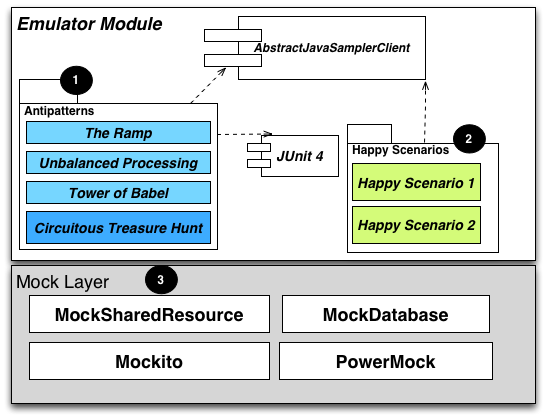
\includegraphics[width=0.5\textwidth]{./images/emulator.png}
\caption{Emulator module}
\label{fig:emulator}
\end{figure}  

\subsection{Test Scenario Library}

This modules provides a common representation for all workloads (Figure \ref{fig:testbedarch}  -\ding{205}). Each workload is composed by a linear vector with 21 positions (Figure \ref{fig:solution}  -\ding{202}). The first position represents an metadata with the name of an individual. The next positions represent 10 scenarios and their numbers of users (Figure \ref{fig:solution}  -\ding{203}). Each scenario is an atomic operation: the scenario must log into the application, run the task goal, and undo any changes performed, returning the application to its original state. 

\subsection{Operation services}

The services are responsible for performing some operations performed by metaheuristics. Figure. \ref{fig:solution} presents the solution representation and an example using the crossover operation. In the example, solution 1 (Figure \ref{fig:solution}  -\ding{204}) has the Login scenario with 2 users, the Search scenario with 4 users, Include scenario with 1 user and the Delete scenario with 2 users.  After the crossover operation with solution 2 (Figure \ref{fig:solution}  -\ding{205}), We obtain a solution with the Login scenario with 2 users, the Search scenario with 4 users, the Update scenario with 3 users and the Include scenario with 5 users (Figure \ref{fig:solution}  -\ding{206}). Figure. \ref{fig:solution} -\ding{207} shows the strategy used by the proposed solution to  obtain the neighbors for the Tabu search and simulated annealing algorithms. The neighbors are obtained by the modification of a single position (scenario or number of users) in the vector.


\begin{figure}[h]
\centering
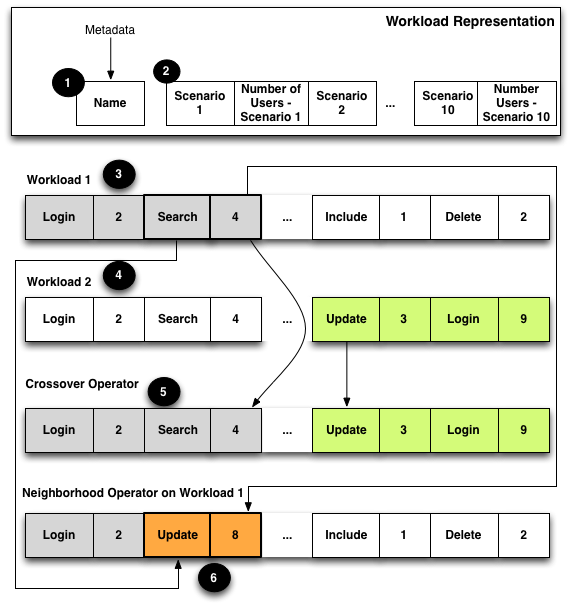
\includegraphics[width=0.5\textwidth]{./images/genomere.png}
\caption{Solution representation, crossover  and neighborhood operators}
\label{fig:solution}
\end{figure}



\section{Experiments}

In this section, We present the results of experiments which we carried out to verify the antipatterns  implementation and the metaheuristics used by the testbed tool. We conducted two experiments in order to verify the effectiveness of the testbed tool. Each experiment use two different antipatterns and the happy scenarios. The experiments ran for 17 generations. The experiments used an initial population of 4 individuals by metaheuristic. The genetic algorithm used the top 10 individuals from each generation in the crossover operation. The Tabu list was configured with the size of 10 individuals and expired every 2 generations.  The mutation operation was applied to 10\% of the population on each generation. The experiments uses tabu search, genetic algorithms and the hybrid metaheuristic approach proposed by Gois et al. \cite{Gois2016}. The objective function applied is intended to maximize the number of users and minimize the response time of the scenarios being tested.  In this experiments, better fitness values means to find scenarios with more users and lower values of a response time. A penalty is applied when the response time is greater than the  maximum response time expected. 

\subsection{Experiment Research Questions}

The following research question is addressed:
\begin{itemize*}
\item Does the IAdapter testbed correctly emulates an antipattern?
\item Does the IAdapter testbed be able to provide metrics with the aim of being used for stress search-based evaluation studies? 
\item Is the IAdapter testbed extensible, allowing the use of several metaheuristic approaches?
\end{itemize*}

\subsection{Variables}

The independent variables are the test scenarios (antipatterns and happy scenarios). The dependent variable are: the number of antipatterns found in best workloads and the metaheuristic with the best fitness value.

\subsection{Hypotheses}

\begin{itemize}
\item With regard to antipatterns implementation or emulation:
\begin{itemize*}
\item $H_{0}$ (A null hypothesis) :the best workloads found in the experiments contain antipatterns
\item $H_{1}$  : the best workloads found in the experiments do not contain antipatterns.
\end{itemize*}
\end{itemize}

\begin{itemize}
\item With regard to metrics provided by the IAdapter:
\begin{itemize*}
\item $H_{0}$ (A null hypothesis) : The IAdapter testbed does not be able to provide metrics with the aim of being used for stress search-based evaluation studies.
\item $H_{1}$  : The IAdapter testbed is able to provide metrics with the aim of being used for stress search-based evaluation studies.
\end{itemize*}
\end{itemize}

\begin{itemize}
\item With regard to the IAdapter testbed customization:
\begin{itemize*}
\item $H_{0}$ (A null hypothesis) :the IAdapter testbed is not extensible, disallowing the use of several metaheuristic approaches.
\item $H_{1}$  : the IAdapter testbed is extensible, allowing the use of several metaheuristic approaches.
\end{itemize*}
\end{itemize}

\subsection{The Ramp and Circuitous Treasure Hunt experiment}

The experiment was carried out for 8 continuous hours.  All tests in the experiment were conducted without the need of a tester, automating the process of executing and designing performance test scenarios.In this experiment, Scenarios were generated with the Ramp and Circuitous Treasure antipattern as well as scenarios with Happy Scenario 1, Happy Scenario 2 and mixed scenarios. Figure \ref{fig:boxplot1} present the fitness value obtained by each metaheuristic.

\begin{figure}[h]
\begin{minipage}{.5\textwidth}
\centering
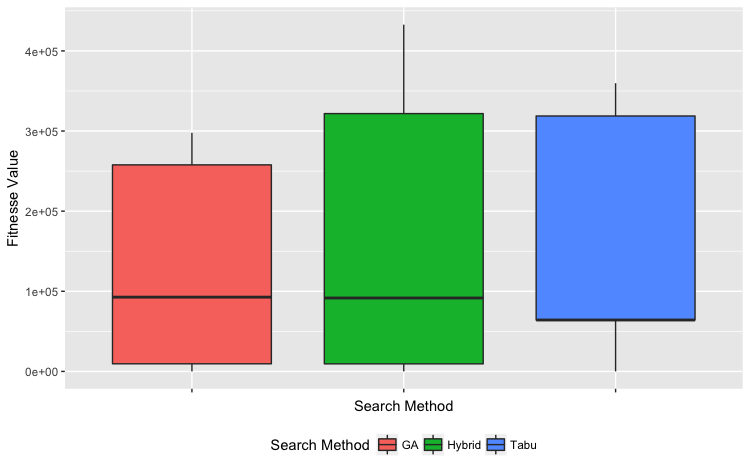
\includegraphics[width=0.8\textwidth]{./images/experiment1-4.png}
\caption{Average, median, maximum and minimal fitness value by Search Method}
\label{fig:boxplot1}
\end{minipage}
\end{figure}

Table \ref{tab:bestindividuals} shows 4 best individuals found in the experiment. None of the best individuals has one of the antipatterns used in the experiment, excluding the scenarios with antipatterns. 

% Please add the following required packages to your document preamble:
% \usepackage[table,xcdraw]{xcolor}
% If you use beamer only pass "xcolor=table" option, i.e. \documentclass[xcolor=table]{beamer}
\begin{table}[h]
\centering
\caption{Best individuals found in the first experiment}
\label{tab:bestindividuals}
\begin{tabular}{lllll}
\rowcolor[HTML]{C0C0C0} 
\textbf{Metaheur.} & \textbf{Gen.} & \textbf{Users} & \textbf{Fit} & \textbf{Scenarios}  \\
Hybrid & 17 & 145 & 432760 & Happy 1 \& 2  \\
Hybrid & 17 & 145 & 432740 & Happy 1 \& 2   \\
Hybrid & 17 & 146 & 431760 & Happy 1 \& 2  \\
Hybrid & 16 & 143 & 426740 & Happy 1 \& 2  
\end{tabular}
\end{table}


\vspace*{-.075in}
\subsection{The Tower Babel  and Unbalanced Processing experiment}
\vspace*{-.075in}

The experiment was carried out for 6 continuous hours. In this experiment, Scenarios were generated with Tower Babel and Unbalanced Processing antipattern as well as scenarios with Happy Scenario 1, Happy Scenario 2 and mixed scenarios.

\begin{figure}[h]
\begin{minipage}{.5\textwidth}
\centering
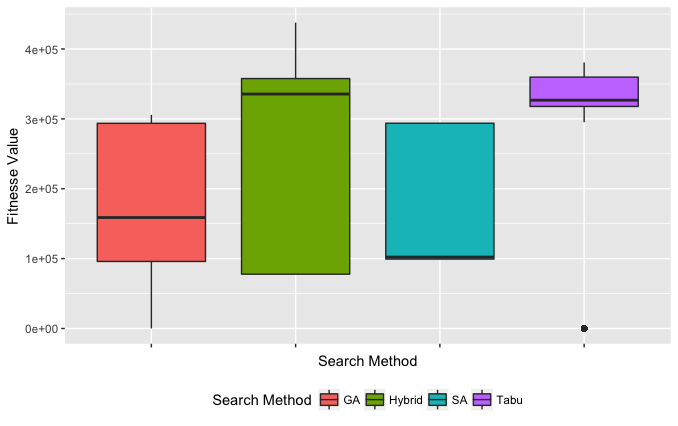
\includegraphics[width=0.8\textwidth]{./images/experiment2-2.png}
\caption{Finesse value by generation in all tests}
\label{fig:boxplot2}
\end{minipage}

\end{figure}



Table \ref{tab:bestindividuals2} shows the 4 best workloads found in the second experiment. Despite the fact of doing 300 conversions of the JSON format to XML. The antipattern implementation does not return a higher response time than happy paths. While happy paths returns from 10 to 15 seconds from a single user, Tower Babel antipattern has a response time of 10 to 29 seconds. None of the best individuals found implements the Unbalanced Processing antipattern.


% Please add the following required packages to your document preamble:
% \usepackage[table,xcdraw]{xcolor}
% If you use beamer only pass "xcolor=table" option, i.e. \documentclass[xcolor=table]{beamer}
\begin{table}[h]
\centering
\caption{Best individuals found in the second experiment}
\label{tab:bestindividuals2}
\begin{tabular}{lllll}
\rowcolor[HTML]{FFCCC9} 
\textbf{Metaheur.} & \textbf{Gen.} & \textbf{Users} & \textbf{Fit} & \textbf{Scenarios}  \\ 
\multicolumn{1}{l}{Hybrid} & \multicolumn{1}{l}{17} & \multicolumn{1}{l}{148} & \multicolumn{1}{l}{437780} & \multicolumn{1}{l}{Happy 1,2 \& Tower}  \\ 
\multicolumn{1}{l}{Hybrid} & \multicolumn{1}{l}{17} & \multicolumn{1}{l}{145} & \multicolumn{1}{l}{432740} & \multicolumn{1}{l}{Happy 1,2 \& Tower}  \\ 
\multicolumn{1}{l}{Hybrid} & \multicolumn{1}{l}{16} & \multicolumn{1}{l}{146} & \multicolumn{1}{l}{431800} & \multicolumn{1}{l}{Happy 1,2 \& Tower} \\ 
\multicolumn{1}{l}{Hybrid} & \multicolumn{1}{l}{17} & \multicolumn{1}{l}{145} & \multicolumn{1}{l}{428780} & \multicolumn{1}{l}{Happy 1,2 \& Tower}  \\ 
\end{tabular}
\end{table}

In the second experiment, the metaheuristics converged to scenarios with a happy path and Tower Babel antipattern, excluding the scenarios with Unbalanced Processing antipattern. The hybrid metaheuristic returned individuals with higher fitness scores. The SA algorithm obtained the worst fitness values. 

\subsection{Threats to validity}
\begin{itemize*}
\item Construct Validity: 
In this work, we just evaluate the use of four antipatterns. However, several antipatterns could be applied.  The testbed's common representation and the strategies used for crossover and neighborhood operators need of a better design, using an abstraction pattern to contemplate a major number of possible solutions.
\item Conclusion Validity: 
The Tower Babel antipattern was not excluded by the metaheuristics used in the experiment, requiring new studies with new approaches and experiments.
\end{itemize*}




\vspace*{-.075in}
\section{Conclusion}
\vspace*{-.075in}

IAdapter Testbed is an open-source facility that provides software tools for search based test research. The testbed tool emulates test scenarios in a controled environment using mock objects and implementing performance antipatterns.  Two experiments were conducted to validate the proposed approach. The experiments use genetic, algorithms, tabu search, simulated annealing and a new hybrid approach proposed by Gois et al. \cite{Gois2016}. In the first experiment, none of the best workloads has one of the antipattern scenarios. In the second experiment,  the metaheuristics converged to scenarios with an happy path and Tower Babel antipattern, excluding the scenarios with Unbalanced Processing antipattern. In both experiments the hybrid metaheuristic returned individuals with higher fitness scores. Future works include the use of new antipatterns and more experiments with the use of the Tower Babel antipattern.
% begin experiment section
%%!TEX root=../seke.tex
% mainfile: ../seke.tex

\begin{table}[t]
  \centering

  {\footnotesize
  \begin{tabular}{r | c c c}
                           Schema & Tables & Columns & Constraints \\ \hline
    BioSQL                        & 28     & 129     & 186 \\
    Cloc                          & 2      & 10      & 0 \\
    iTrust                        & 42     & 309     & 134 \\
    JWhoisServer                  & 6      & 49      & 50 \\
    NistWeather                   & 2      & 9       & 13 \\
    NistXTS748                    & 1      & 3       & 3 \\
    NistXTS749                    & 1      & 3       & 3 \\
    RiskIt                        & 13     & 57      & 36 \\
    UnixUsage                     & 8      & 32      & 24
\end{tabular}}

  \vspace*{-.05in}
  \caption{Database schemas used in the experiments.}~\label{tab:schemas}
  \vspace*{-.25in}

\end{table}

\vspace{-.05in}
\section{Empirical Analysis}
\vspace{-.05in}

\textbf{Experimental Design}. To gain a full picture of the performance trade-offs, we conducted an experiment for every
configuration of the parameter space (i.e., schema, coverage criterion, data generator, and doubling technique).
Table~\ref{tab:schemas} shows that the experiments focused on nine
database schemas containing between 1 and 42 distinct
tables, 3 to 309 columns, and up to 186 constraints. Including all of the test adequacy criteria proposed by McMinn et
al.~\cite{mcminn2015}, the experiments study ``weak'' criteria (i.e., APC, NCC, ICC, and UCC), ``moderately strong''
ones (i.e., ANCC, AICC, and AUCC), and ``strong'' criteria (i.e., CondAICC and ClauseAICC). More details about each
criterion, including its formal definition and relationship to the other
criteria, are available in prior work~\cite{mcminn2015}. We
used all six test data generators provided by the {\em SchemaAnalyst} tool for automated test data
generation~\cite{kapfhammer2013}, with four techniques employing a variant of random search and two based on Korel's
alternating variable method. After a restart of the search, each data generator could
start with either default or random values.

% GMK NOTE: Can we safely cut this sentence? I don't think that it is absolutely needed (I have already revised it)

% In an effort to ensure good picks for parameters, we also conducted preliminary experiments.

In our study, we set $\mathit{tolerance}$ to $0.40$ and $\mathit{lookback}$ to $4$. These values were chosen by
performing doubling experiments on various algorithms, with known worst-case time complexities, and observing that the
ratio converged to the correct value with this configuration.  After observing that \textit{SchemaAnalyst} stopped
displaying constant behavior after around five doubles, we set
$\mathit{minimum}$ to be four times this number.
Preliminary studies showed that, while experiments for ``fast'' configurations could be completed in less than an hour,
``slower'' configurations required days.  Since there are over two thousand possible configurations, the study needed
a substantial amount of computational resources.  As a solution, we ran the experiments on a high-performance computing
(HPC) cluster containing 195 worker nodes of various hardware configurations, ranging from 12 to 16 CPU cores and 24 to
256 GB of memory, and using a 64-bit GNU/Linux operating system.

% GMK NOTE: It would be better to call this a tree model instead of a regression tree -- the word regression is also
% used in the software testing literature to have a different meanining.

% Regression tree
% Belongs with results_trees, but must be here for page placement within the paper

%%!TEX root=seke.tex
% mainfile: ../seke.tex

\textbf{Results}. Our experiments reveal that, when doubling \texttt{UNIQUE}s, {\tt NOT NULL}s, and {\tt CHECK}s,
\textit{SchemaAnalyst} displays linear or linearithmic worst-case time complexity.  Out of the 699 experiments performed
to double these schema structures, $72\%$ converged to linear or linearithmic.  Another $8\%$ failed to converge, and of
these experiments, $80\%$ failed because of memory limitations, $13\%$ exceeded the maximum time limit, and $8\%$ failed
for reasons that could not be determined.  The doubling ratios among these experiments were primarily linear or
linearithmic at the time they were terminated, however there were $14$ that were quadratic and $3$ that were cubic.  The
experiments that failed to converge were primarily generating test data for complex schemas, such as iTrust and BioSQL,
and the most stringent adequacy criteria, such as ANCC and AUCC. The remaining $20\%$ of the 699 experiments converged
on constant or logarithmic.  Since there did not seem to be a pattern in which configurations converged this way
compared to linear or linearithmic, it is likely that they terminated before the true worst-case time complexity was
apparent.

\begin{figure}[t]
\centering
  \centering
  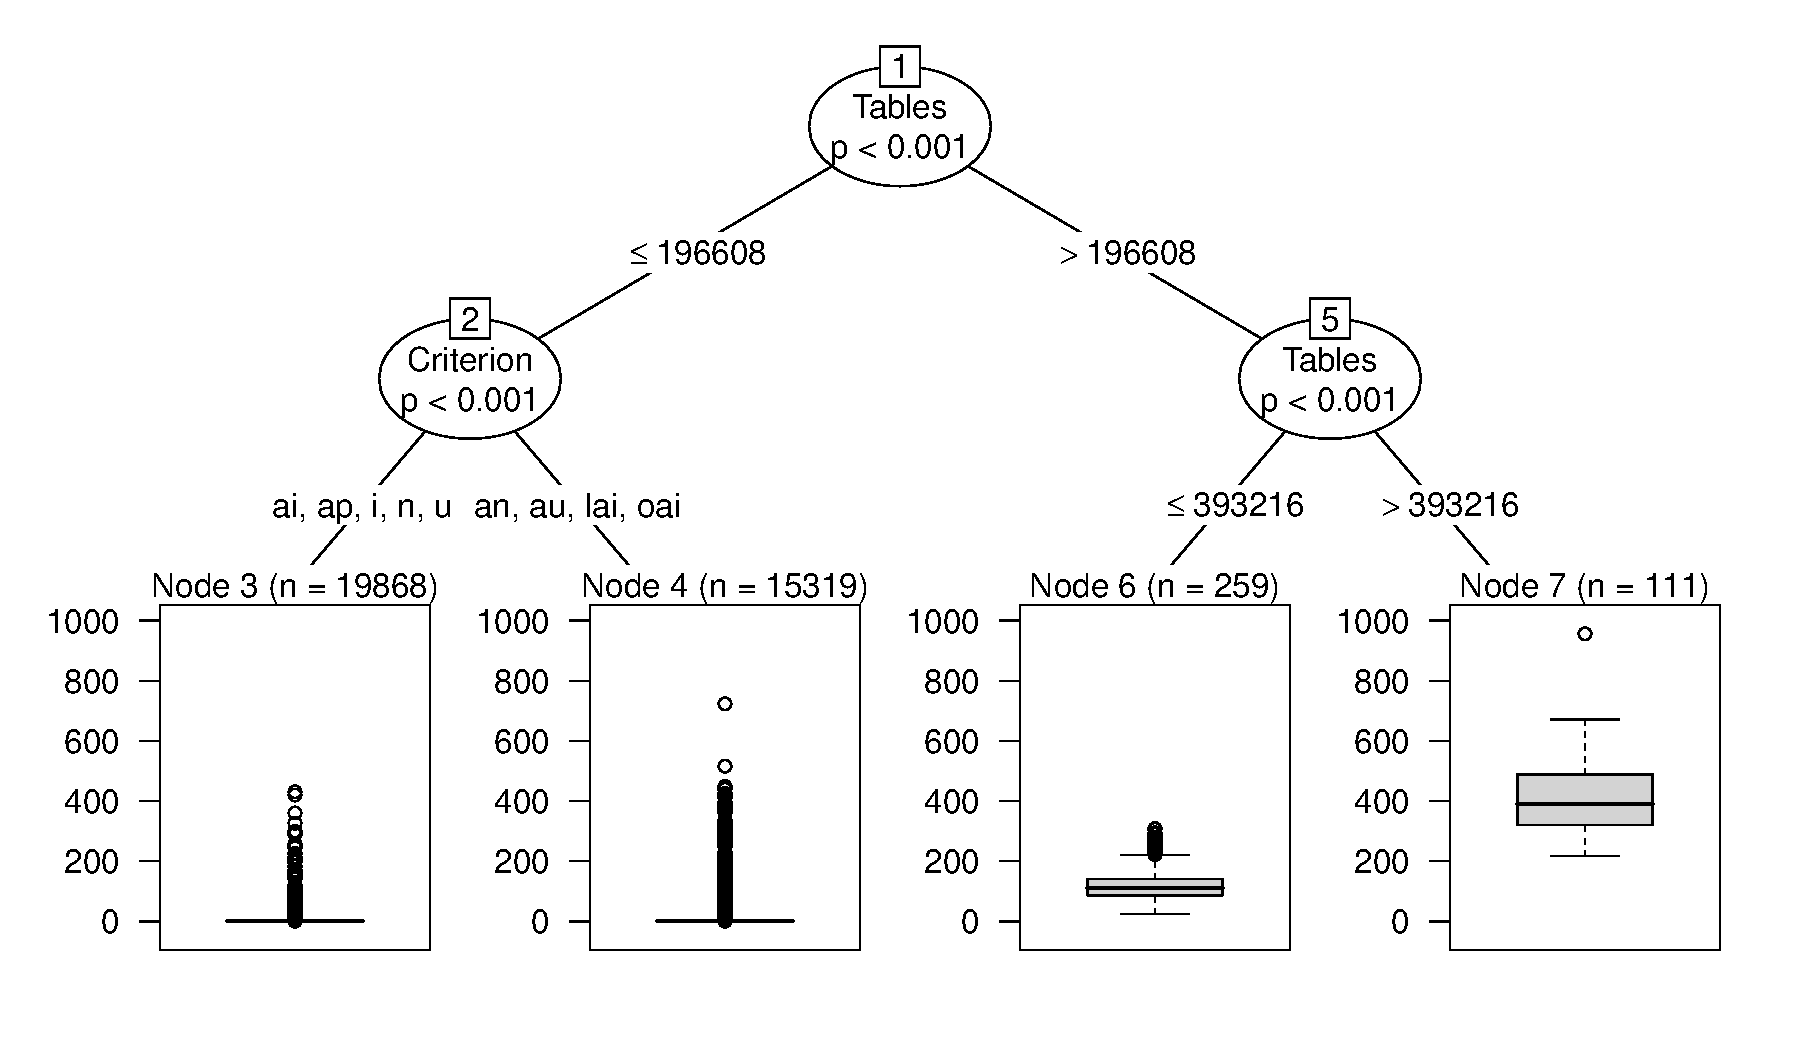
\includegraphics[width=1.025\linewidth]{diagrams/Tree.pdf}
  \vspace*{-.25in}
  \caption{Tree model using all variables to predict runtime in minutes,
  demonstrating the important of the table count. \\ Due to space
  constraints, criterion names are abbreviated.
  \vspace{-.35in}}~\label{fig:atree}
\end{figure}

When doubling the tables and columns in the schemas, the results were less conclusive. Doubling the number of tables in
the schema caused the runtime of \textit{SchemaAnalyst} to increase much faster than it did for the other integrity
constraints. As a result, $56\%$ of the 467 experiments doubling this schema feature were terminated before convergence
because they exceeded the time limit.  Of the experiments that converged, 72 converged to quadratic and 10 converged to
cubic.  Of the experiments that terminated before they converged, the doubling ratios for 205 indicated quadratic, 18
suggested cubic, and 37 were worse than cubic.

Experiments on the number of columns were also inconclusive.  We noted that 208 of the converged experiments showed
linear or linearithmic time complexity, while 28 converged to quadratic and 2 cubic.  Another 203 experiments failed to
converge; however, unlike the experiments that doubled the number of tables, the experiments for doubling the number of
columns most frequently failed by running out of memory rather than exceeding the time limit. The experiments that did not
converge included 106 ratios indicating quadratic behavior, 73 cubic, and 3 worse.

% CBK NOTE: moved them back, they really want to be in this file

\begin{figure*}[t!]
\vspace*{-.28in}
\centering
\begin{subfigure}{0.5\textwidth}
  \centering
  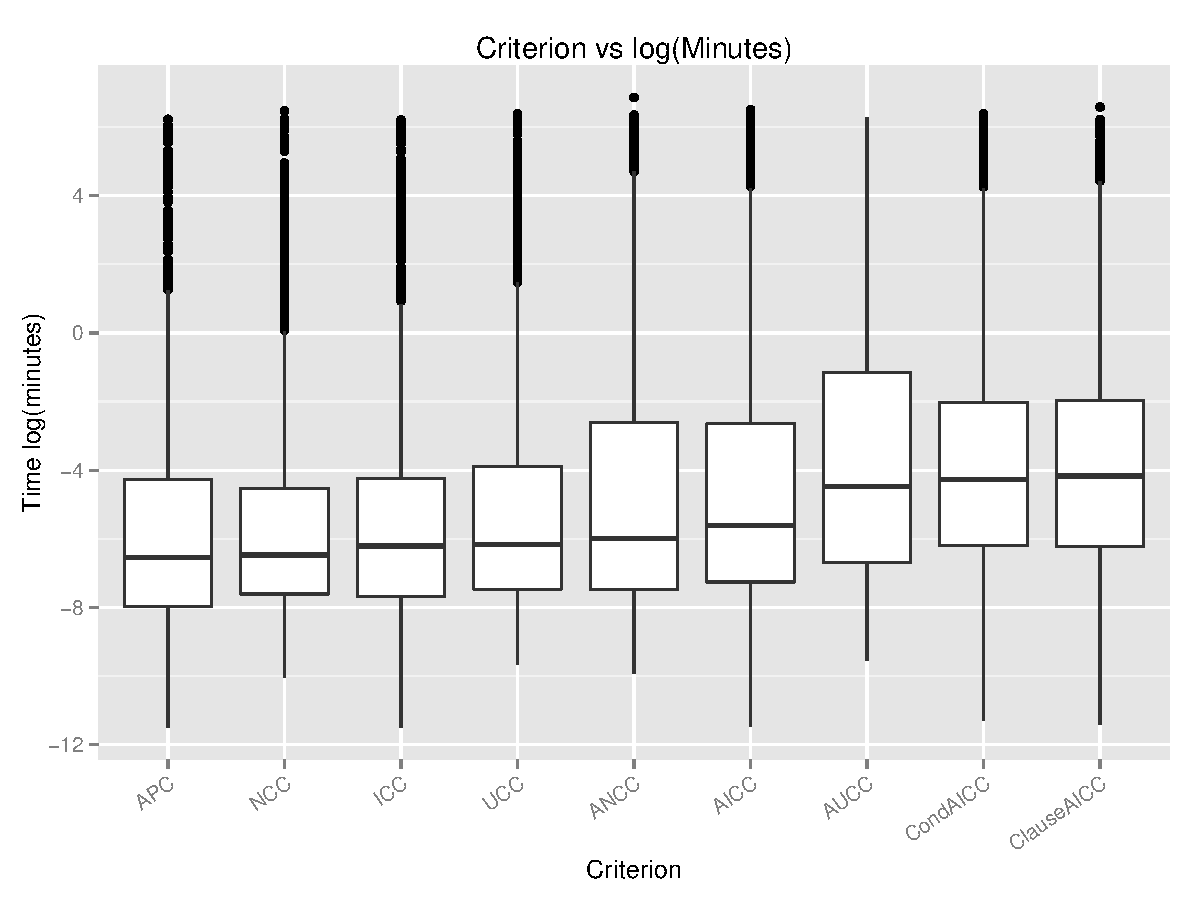
\includegraphics[width=.77\linewidth]{diagrams/CriterionOrder.pdf}
  \caption{Coverage criterion versus runtime in minutes.}
  \label{fig:crites}
\end{subfigure}%
\begin{subfigure}{0.5\textwidth}
  \centering
  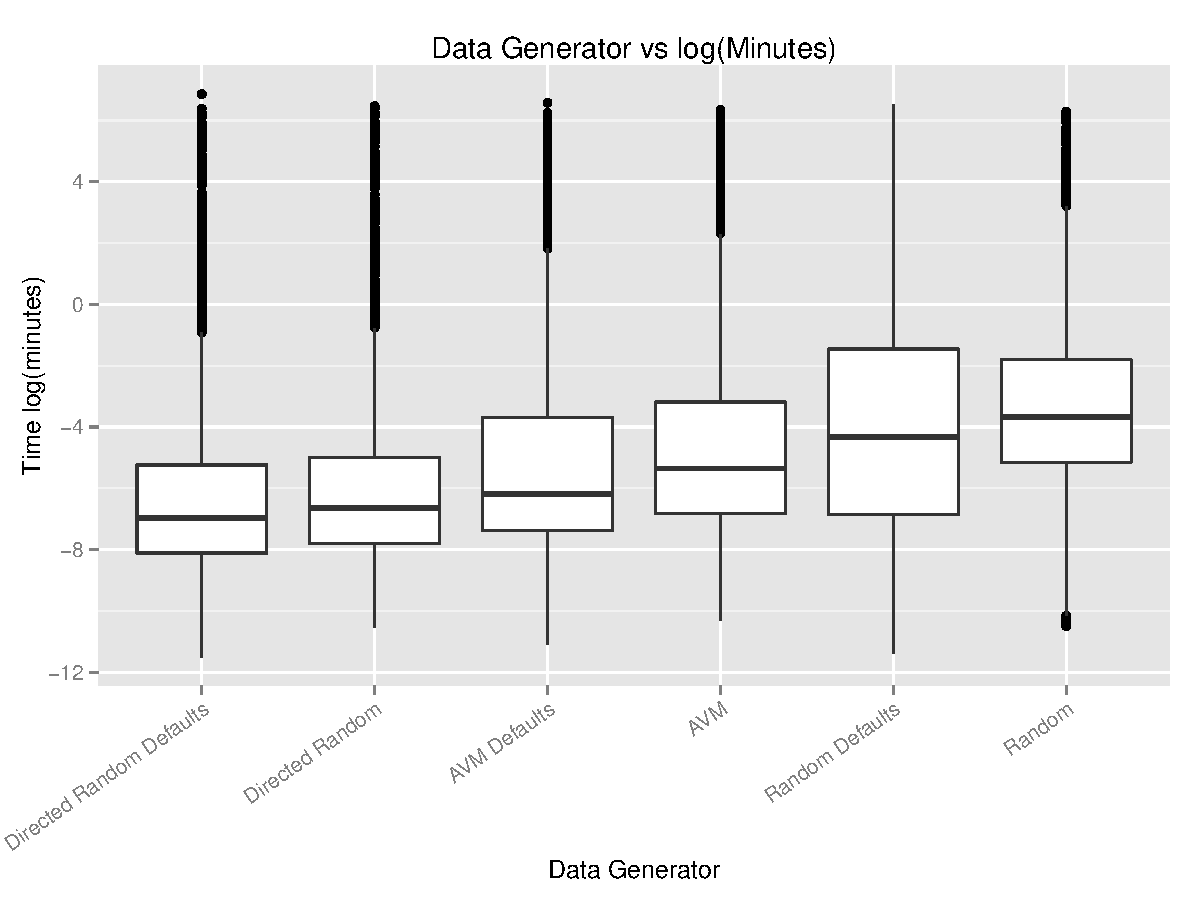
\includegraphics[width=.77\linewidth]{diagrams/DataGeneratorOrder.pdf}
  \caption{Data generator versus runtime in minutes.}
  \label{fig:datas}
\end{subfigure}
\label{fig:bwplots}
\caption{Box and whisker plots for criterion and data
  generator.}
  \vspace*{-.15in}
\end{figure*}

% GMK NOTE: These have now been moved to another file!

% Box and whisker plots
% Belongs to results_bwplots, but must be here for positioning reasons

%% vim: ft=tex
%!TEX root=seke.tex
% mainfile: ../seke.tex

To gain a more nuanced understanding of the results, our tool constructed a conditional inference tree model using the
\textit{ctree} package in the R language. These trees use the values of predictor variables (e.g., the adequacy
criterion) to model the value of a response variable (e.g., {\em SchemaAnalyst}'s runtime);~\textit{ctree} accomplishes this
by repeatedly splitting the data according to what predictor variable has the most influence on the response variable.
Each tree node represents a choice of predictor variable, and the level of the node indicates its importance to
the prediction, with higher nodes being more important to predicting generation time.

% \textit{ctree} produced the tree shown as Figure~\ref{fig:atree} to predict the runtime of \textit{SchemaAnalyst} with
% the predictor variables: tables, columns, {\tt UNIQUE}s, {\tt NOT NULL}s, {\tt CHECK}s, chosen criterion, and the data
% generator.  The regression tree confirms that the number of tables has the greatest impact on runtime, and also reveals
% that when the number of tables in the schema is small, the choice of coverage criterion is most significant.

% \textit{ctree} produced the tree shown as Figure~\ref{fig:atree} to predict the runtime of \textit{SchemaAnalyst} with

Using predictor variables for the number of tables, columns, {\tt UNIQUE}s, {\tt NOT NULL}s, and {\tt CHECK}s; and the
chosen criterion and data generator, \textit{ctree} produced the tree model in Figure~\ref{fig:atree}.  In addition to
confirming that the number of tables has the greatest impact on runtime, the tree also reveals that, when the number of
tables in the schema is small, the choice of coverage criterion is most
significant.  While the number of tables had a large impact when over $197,000$, in practice schemas are unlikely to be this large. Another invocation of
\textit{ctree}, excluding tables from the list of predictors, provided insight into the behavior of
\textit{SchemaAnalyst} for more practical table sizes. In this tree, not shown due to space constraints, the coverage
criterion emerged as the most important predictor for runtime, followed by the choice of data generator, and then the
number of columns.

%% vim: ft=tex
%!TEX root=seke.tex
% mainfile: ../seke.tex

While the trees provide insight into the relative impact of each predictor, the box and whisker plots shown in the
leaves of the trees do not furnish a detailed view of the choices within each predictor.  To gain a finer-grained
understanding, we created box and whisker plots of our own:  Figure~\ref{fig:crites} shows the influence of coverage
criterion on runtime, while Figure~\ref{fig:datas} shows the effect of data generator on runtime.
Figure~\ref{fig:crites} shows that the strongest coverage criteria in the subsumption hierarchy (i.e., AUCC, ClauseAICC,
and CondAICC) cause runtime to increase the most, followed by ANCC and AICC, and then the remaining criteria (i.e., APC
through UCC).  We anticipate that the stronger criteria always lead to higher time overheads because they force {\em
SchemaAnalyst} to generate more tests.  Also, criteria at the same level in the hierarchy engender similar runtimes.

Figure~\ref{fig:datas} reveals that, by a substantial margin, the Random and Random Defaults generators took the most
time to generate data. This counterintuitive result suggests that less effective data generators actually take longer to
create data than those that are known to be more effective~\cite{kapfhammer2013}.  A less pronounced difference between
the remaining generators can be observed, with the use of default values consistently being faster than the use of
random values at restart.

\begin{table*}[th]
\vspace*{-.2in}
  \centering
  \small
\begin{tabular}{llllllllll}
           & APC      & ANCC     & CondAICC & NCC      & AUCC     & AICC     & ClauseAICC & ICC      & UCC   \\
APC        & NA       & \cellcolor{gray!25}0.425    &
\cellcolor{gray!45}0.337    & 0.484    &\cellcolor{gray!45} 0.334    &
\cellcolor{gray!25}0.413    &\cellcolor{gray!45} 0.329      & 0.481    & 0.449 \\
ANCC       & 2.20E-16 & NA       &\cellcolor{gray!25} 0.407
&\cellcolor{gray!25} 0.561    &\cellcolor{gray!25} 0.405    & 0.484
&\cellcolor{gray!25} 0.399      & 0.554    & 0.526 \\
CondAICC   & 2.20E-16 & 2.20E-16 & NA       &\cellcolor{gray!45} 0.671
& 0.503    &\cellcolor{gray!25} 0.581    & 0.492
&\cellcolor{gray!45} 0.656    &\cellcolor{gray!25} 0.634 \\
NCC        & 1.20E-02 & 2.20E-16 & 2.20E-16 & NA
&\cellcolor{gray!45} 0.335    &\cellcolor{gray!25} 0.417
&\cellcolor{gray!45} 0.322      & 0.491    & 0.461 \\
AUCC       & 2.20E-16 & 2.20E-16 & \fbox{6.92E-01} & 2.20E-16 & NA       &
\cellcolor{gray!25}0.577    & 0.490      &\cellcolor{gray!45} 0.651
&\cellcolor{gray!25} 0.628 \\
AICC       & 2.20E-16 & 1.70E-02 & 2.20E-16 & 2.20E-16 & 2.20E-16 & NA
&\cellcolor{gray!25} 0.412      &\cellcolor{gray!25} 0.571    & 0.547 \\
ClauseAICC & 2.20E-16 & 2.20E-16 & \fbox{2.72E-01} & 2.20E-16 & 1.40E-01 &
2.20E-16 & NA         & \cellcolor{gray!45}0.662    &\cellcolor{gray!45} 0.641 \\
ICC        & 4.00E-03 & 2.20E-16 & 2.20E-16 &\fbox{1.83E-01} & 2.20E-16 & 2.20E-16 & 2.20E-16   & NA       & 0.472 \\
UCC        & 9.30E-16 & 3.83E-05 & 2.20E-16 & 7.36E-10 & 2.20E-16 &
5.73E-13 & 2.20E-16   & 9.29E-06 & NA    \\ \hline
& Rank-Sum: & significant & \fbox{insignificant} & &
$\hat{A}_{12}$: & none & \cellcolor{gray!25} small &
\cellcolor{gray!45} medium & \cellcolor{gray!65} large
\end{tabular}

\caption{For each pair of coverage criteria, lower left shows Wilcoxon Rank-Sum Test, upper right shows $\hat{A}_{12}$.}
\label{tab:crites}
\vspace*{-.2in}
\end{table*}

%% vim: ft=tex
%!TEX root=seke.tex
% mainfile: ../seke.tex

While the box and whisker plots show how choices between coverage criteria and data generators affect runtime, the
question remains if these differences are statistically and practically significant. To answer this question, we employ
the Wilcoxon rank-sum test and the $\hat{A}_{12}$ effect size~\cite{mcminn2015}.

The Wilcoxon rank-sum test is a non-parametric test for hypothesis testing.  If the result of the test is greater than
the significance level ($0.05$ is frequently used), then the configurations are indistinguishable.  If, however, the
result is less than the chosen level, then they are different.  The $\hat{A}_{12}$ test is similar, but for drawing
conclusions about the practical difference between two collections of data.  A result of $\hat{A}_{12}=0.50$ means that
any difference is not practically significant, while $\hat{A}_{12}>0.56$ or $<0.44$ signifies a small difference,
$\hat{A}_{12}>0.64$ or $<0.36$ denotes a medium difference, and $\hat{A}_{12}>0.71$ or $<0.29$ indicates a large
difference.

Table~\ref{tab:crites} shows the statistical tests calculated for every pair of coverage criteria. The Wilcoxon
rank-sum test reveals that changing the criterion results in statistically significant differences in runtimes, with the
exception of changing between the four criteria at the top of the subsumption hierarchy and the two criteria at the
bottom.  The $\hat{A}_{12}$ results generally show a small to medium practical effect size when switching between
criteria at the high or low end of the hierarchy, and small or no effect when switching between criteria at the same
level of the hierarchy.

The statistical tests were calculated for all pairs of data generators, but the resulting table was omitted due to space
constraints. All comparisons of data generators were statistically significant according to the Wilcoxon rank-sum test.
The $\hat{A}_{12}$ values show that all choices of data generator have at least a small practical impact, with the
exception of choosing between random and random defaults, and directed random and directed random defaults.  Changing
between these data generators results in a large to medium effect size, and comparing either of the AVM-based
generators to the other primarily resulted in a small difference.

%%!TEX root=seke.tex
% mainfile: ../seke.tex

% CBK Note: 'unique' is a poor word choice since it's a constraint name

\textbf{Threats to Validity}. Our technique for doubling the number of constraints in the schema is simply to duplicate
the existing constraints. It is possible that \textit{SchemaAnalyst} does less work processing these redundant
constraints than it would given non-restated ones. However, doubling the constraints in this way is easy to implement
and, as the results show, good at revealing performance trade-offs.  Additionally, since worst-case time is only
apparent for large $n$, it is possible that the experiments terminated too quickly.  While we attempted to configure the
parameters of our tool using algorithms with known worst-case complexities and conducting preliminary experiments with
various settings and under manual supervision, it is possible that our configuration was not optimized for use on the HPC
cluster.


%%!TEX root=../seke.tex
% mainfile: ../seke.tex

\vspace*{-.05in}
\section{Conclusions and Future Work}
\vspace*{-.1in}

% The automated doubling experiment was able to determine the worst case time complexity of \textit{SchemaAnalyst} with
% respect to the number of check constraints in the input schema, for the \textsc{constraintCACCoverage} criterion and the
% \textsc{directedRandom} data generator.  Additional experiments will be conducted on other criteria and data generators.
% Additionally, other factors that may influence the runtime of schema analysis, such as the number of primary keys,
% foreign keys, tables, columns, etc will be investigated.

This paper presented an automated method for empirically suggesting the worst-case time complexity of search-based test
data generation methods. Focusing on the domain of relational database schemas, our approach repeatedly doubles the size
of the input schema and observes the commensurate change in runtime. Although some results are inconclusive, we find
that, in many cases, data generation is linear or linearithmic and, in others, it is quadratic, cubic, or worse.  Our
automated method also revealed that, for all of the test adequacy criteria in the subsumption hierarchy presented by
McMinn et al.~\cite{mcminn2015}, stronger criteria always necessitate more time for test data generation.

Since this paper's technique did not consider the doubling of constraints like {\tt FOREIGN KEY}s, future work will
focus on creating doublers for these unstudied constraints. Additionally, the current doubling mechanism avoids
introducing semantically invalid constraints by restating existing constraints; in future work we plan to implement and
evaluate more realistic ways to double relational schemas. Because certain experiments timed out before converging, we
also want to re-run these configurations with longer time limits and more memory. Finally, we will investigate how
automated parameter tuning, instead of manual tuning before experimentation in a new execution environment, can
support choosing the convergence condition. Ultimately, the combination of the presented framework with the completed
future work will yield an effective way to empirically understand the worst-case time complexity of search-based
test data generation for relational database schemas.



% GMK NOTE: I removed this and moved it into the background section
% %!TEX root=seke.tex
% mainfile: ../seke.tex

% \section{Related Work}

%TODO GMK: We need more of this
% Even if you know of some papers, you can send some to me and I can read them

% Goldsmith et al.~\cite{Goldsmith2007} developed a system to empirically evaluate computational complexly.  Their
% system, \textit{Trend-Prof}, uses code instrumentation to count the number of times each block of code is executed,
% and then groups these blocks by their behavior.  \textit{Trend-Prof} takes in a collection of workloads, user
% specified features of the workloads, and the program to be studied. This technique results in a more powerful
% analysis. However, the authors do not address the issue of generating the workloads necessary to achieve a meaningful
% result, and we attempt to do this automatically.  Additionally, our approach is novel because we apply it to a domain
% where the theoretical scalability is not yet known.


% \titleformat{\chapter}{\huge\bf}{}{10pt}{\arabic{chapter} \ }[\titlerule]
\setlength{\bibitemsep}{.075in}
{\footnotesize
  \bibliographystyle{IEEEtran}
% \vspace*{-.05in}
\bibliography{bibtex/seke}}

\end{document}
